\documentclass[aspectratio=169,xcolor=table]{beamer}

% --- Português do Brasil ---
\usepackage[utf8]{inputenc}
\usepackage[T1]{fontenc}      % acentos e hifenização corretos
\usepackage{lmodern}          % fonte vetorial com suporte a acentos
\usepackage[brazilian]{babel} % hifenização, datas e rótulos em PT-BR

% --- Pacotes e comandos usados em tabela_beamer.tex ---
\usepackage{booktabs}
\usepackage{multirow}
\usepackage{pifont}
\usepackage{array}

\newcommand{\cmark}{\ding{51}}
\newcommand{\xmark}{\ding{55}}

% --- Comandos usados em gramatica_beamer.tex ---
% Tokens especiais (NEWLINE, INDENT, DEDENT) em negrito sem serifa
\newcommand{\tok}[1]{\mbox{\textsf{\textbf{#1}}}}
% Barra que separa as alternativas da BNF
\newcommand{\ou}{$\mid$\ }

% Cabeçalho da tabela reutilizado em todos os slides
\newcommand{\cabecalho}{%
  \toprule
  \multirow{2}{*}{\textbf{Problema de benchmark}} &
  \multicolumn{2}{c}{\textbf{Taxa de sucesso}} &
  \multirow{2}{*}{\textbf{Iter./Recur.}} \\
  \cmidrule(lr){2-3}
  & \textbf{Mediana (IQR)} & \textbf{Máx.} & \\
  \midrule
}

% Legenda da tabela, exibida abaixo da tabela em cada slide
\newcommand{\legenda}{%
  \par\vspace{0.6em}
  {\footnotesize
    \textbf{Tabela:} taxas de sucesso em \% \cite{survey}. \textbf{Mediana (IQR)}: mediana da taxa de
   sucesso e intervalo interquartil; \textbf{Máx.}: maior taxa de sucesso observada.
   \textbf{Iter./Recur.}: \cmark~= usa iteração/recursão; \xmark~= não usa.\par.}
}

\usetheme{default}
\usecolortheme{default}
\setbeamertemplate{navigation symbols}{}
\title{A Comprehensive Survey on Program Synthesis With Evolutionary Algorithms}
\institute{Metodologia de Pesquisa - 2026.3 \\
Pós-graduação em Ciência da Computação - UFABC}
\author{Pedro Moreno Silva}
\date{\today}

% OK - O que é síntese de programas?
% OK -  que é programação genética?
% OK - Como identificaram as representações mais usadas em GP?
% OK - O que é Stack-based GP?
% OK - O que é Grammar-guided GP?
% OK - O que é Linear GP e outros?
% OK - O que é o PSB1?
% Como os GPs resolvem os problemas dos benchmarks? (tabela)
% Conclusões tiradas pelos autores
% Trabalhos futuros dos autores


\begin{document}

\begin{frame}
  \titlepage
\end{frame}

\begin{frame}{Conteúdos}
  \tableofcontents
\end{frame}


\section{Conceitualização}

\subsection{Síntese de Programas}
\begin{frame}{O que é Síntese de Programas (SP)?}
    \begin{itemize}
      \item Processo de descoberta automático de programas \cite{gulwani2017}.
      \item \textit{Sem interferência humana!}
    \end{itemize}
\end{frame}

\begin{frame}{Caracterização de SP}
    \begin{itemize}
        \item Podemos caracterizar um sistema de Síntese de Programas sob 3 eixos \cite{gulwani2010}:
        \begin{itemize}
            \item Forma da especificação do problema (ou como o usuário representa sua intenção).
            \item Espaço de busca (todos os programas possíveis em uma dada representação).
            \item Heurística de busca (como navegar o espaço dos programas).
        \end{itemize}
    \end{itemize}
\end{frame}

\subsection{Programação Genética}
\begin{frame}{O que é Programação Genética (GP)?}
        \begin{itemize}
          \item Variação de algoritmos genéticos \cite{kozabook1}.
            \item Heurística baseada na ideia de evolução do mais apto.
            \item Indivíduos são programas, conjuntos de instruções seus genes.
            \item Indivíduos que produzem resultados melhores se reproduzem.
            \item Utilizado como técnica de busca em SP.
        \end{itemize}
\end{frame}
\begin{frame}{O que é Programação Genética (GP)?}
        \begin{figure}
            \centering
            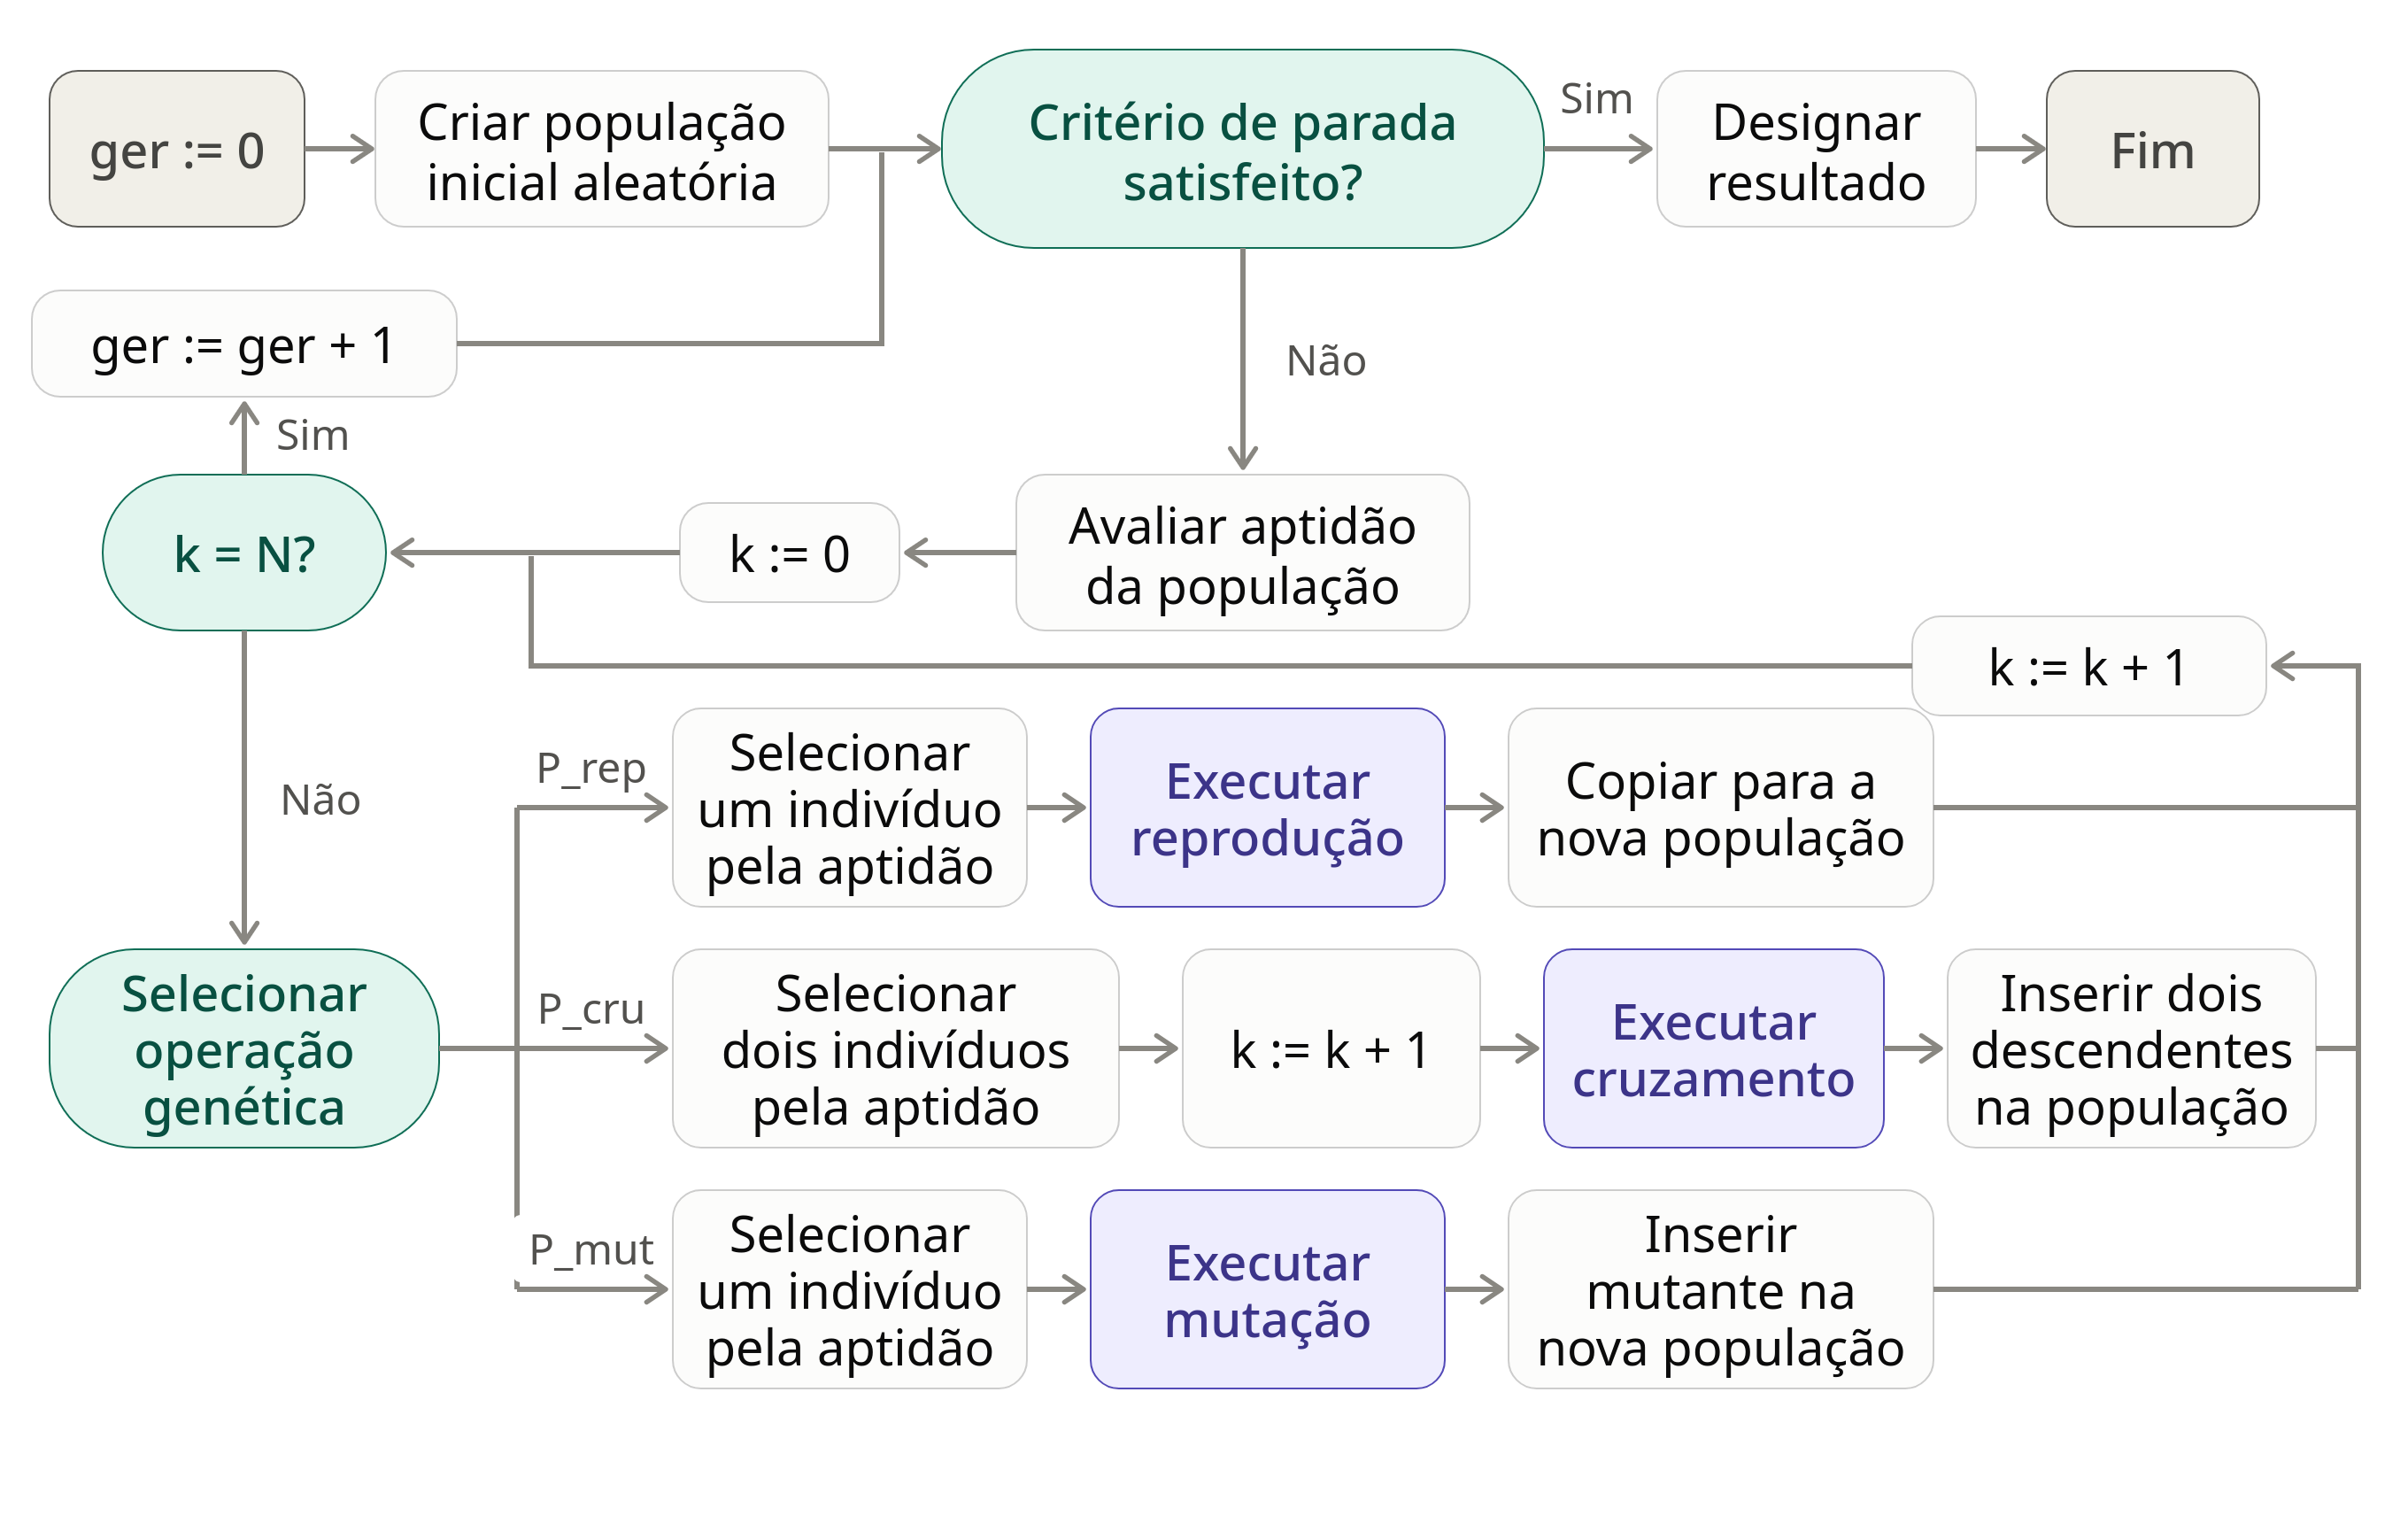
\includegraphics[width=0.7\linewidth]{imgs/flow.png}
            \caption{Fluxograma de GP. Adaptado de \cite{kozabook1}}
            \label{fig:flow}
        \end{figure}
\end{frame}
\begin{frame}{O que é Programação Genética (GP)?}
  \begin{columns}
    \begin{column}{0.5\textwidth}
      \begin{figure}
          \centering
          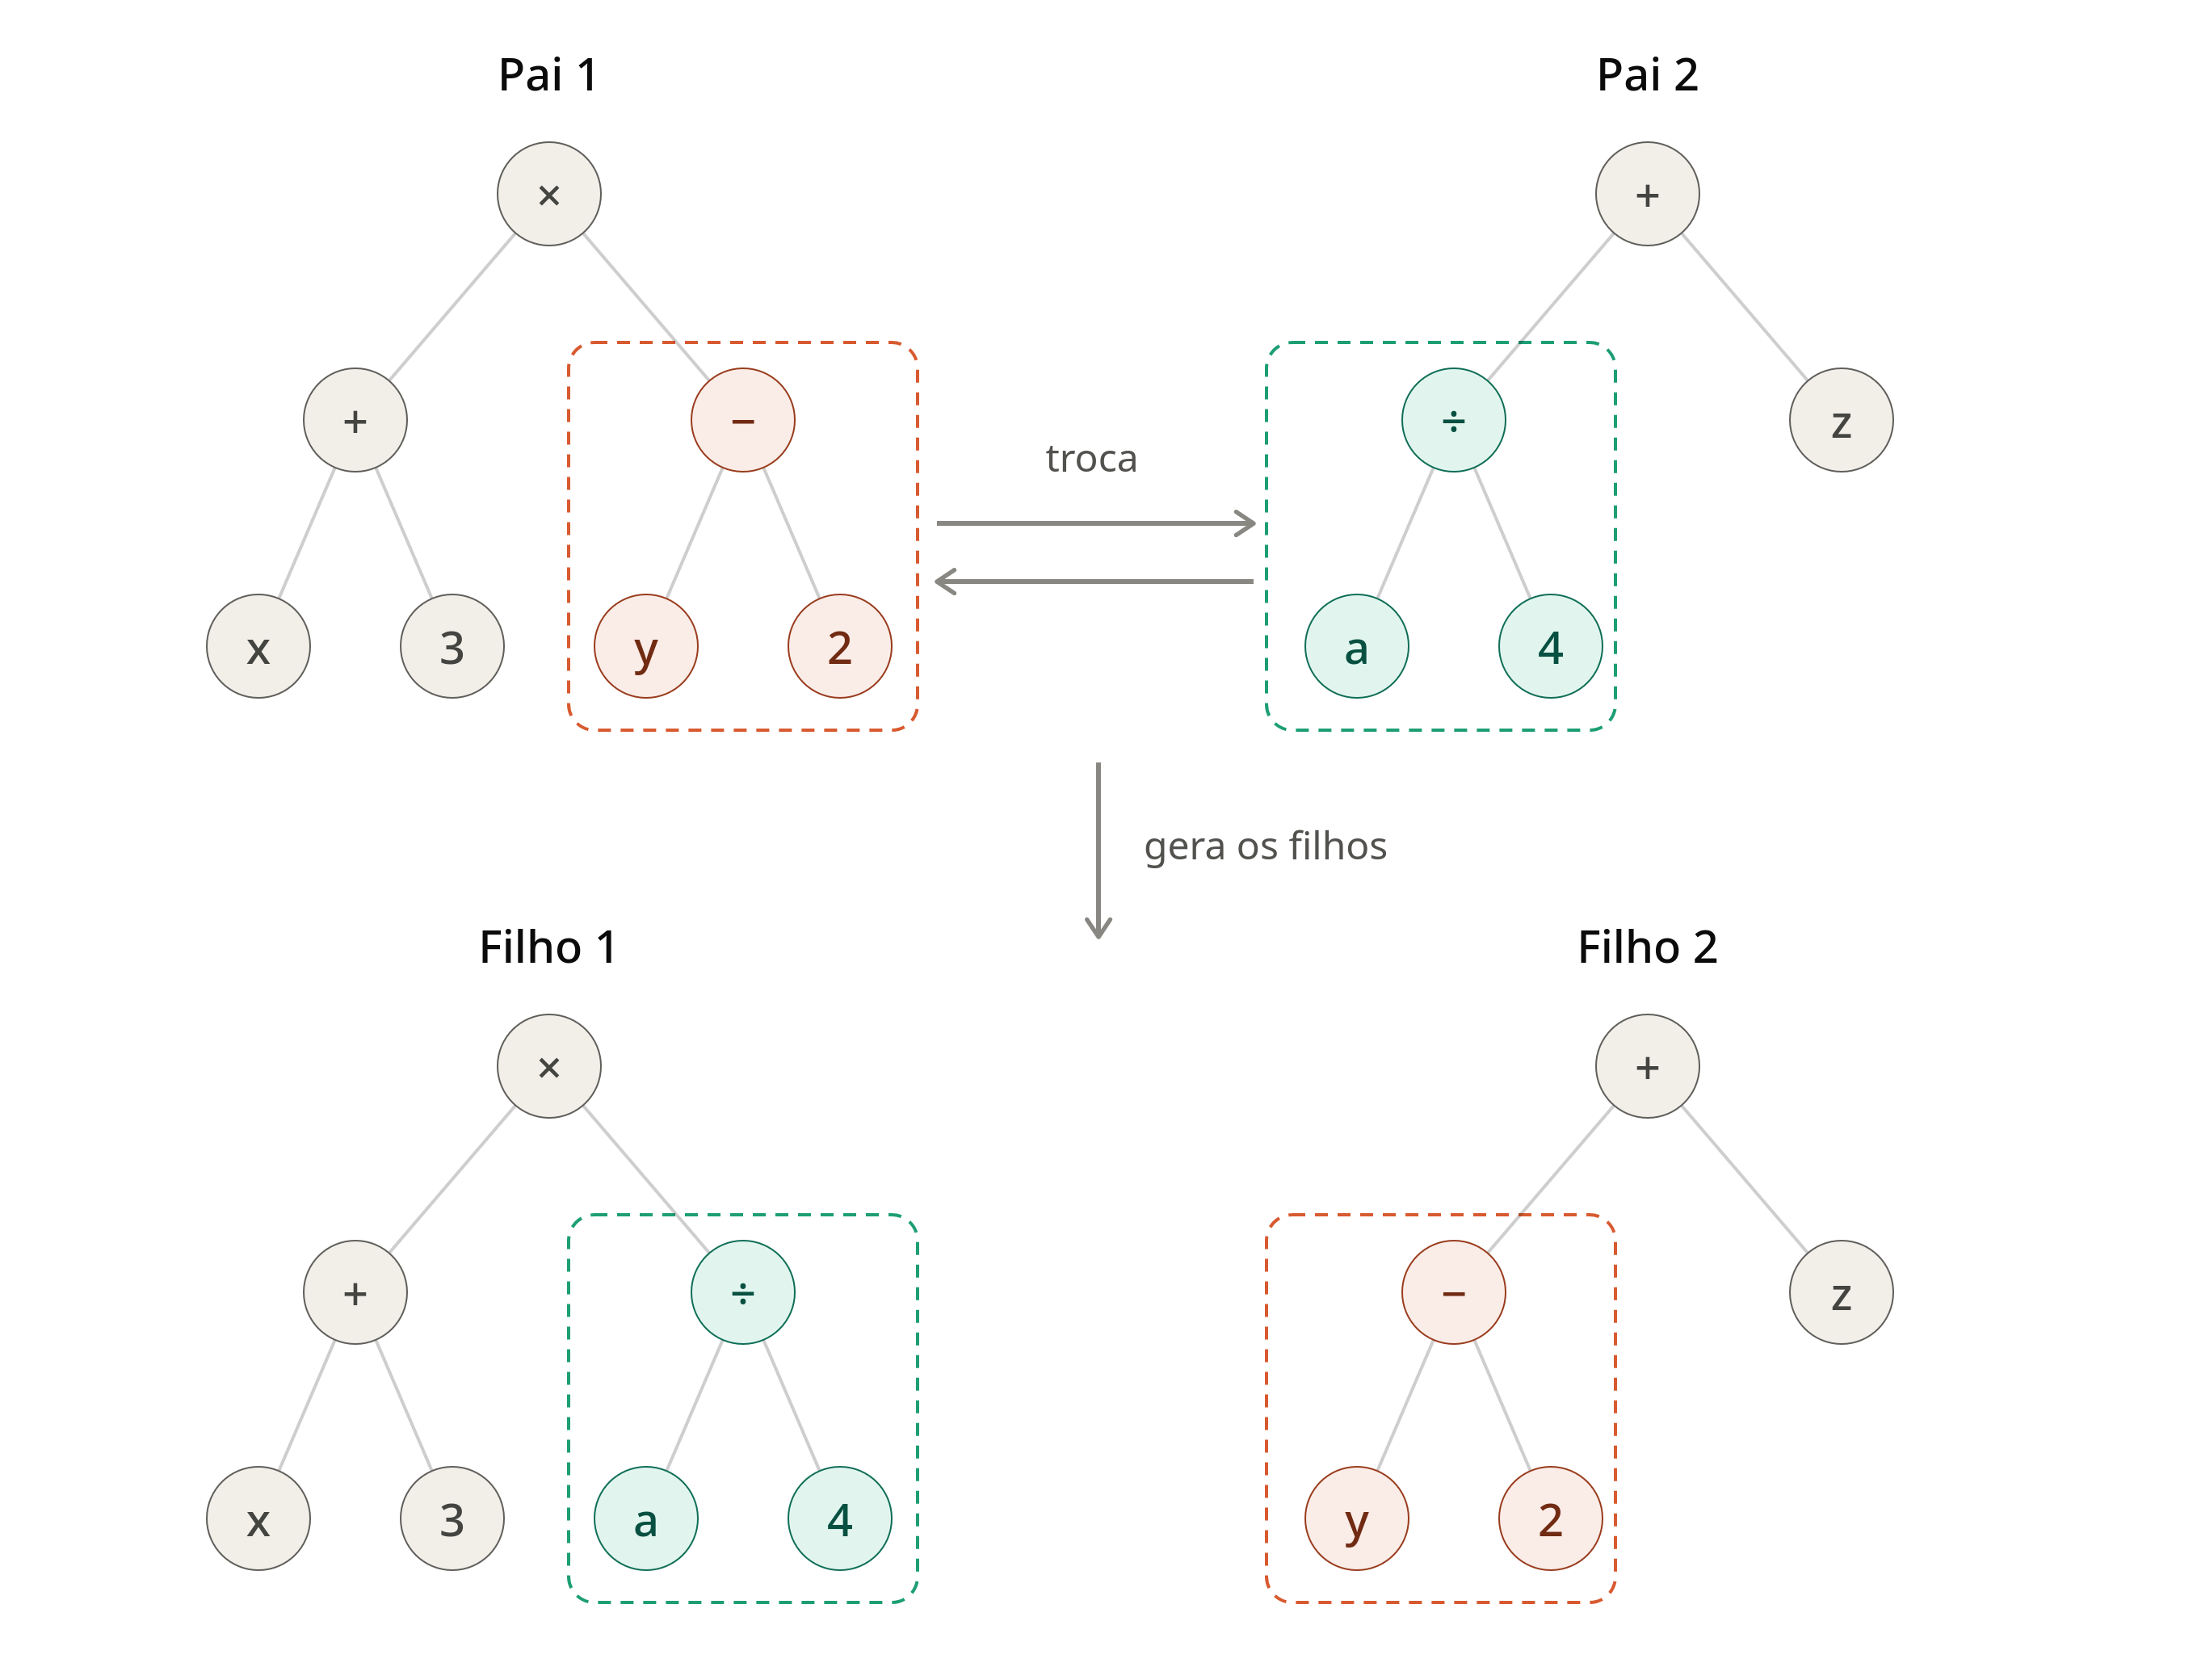
\includegraphics[width=\linewidth]{imgs/crossover.png}
          \caption{Operador de \textit{crossover}. Adaptado de \cite{koza1994}}
          \label{fig:cx}
      \end{figure}
    \end{column}

    \begin{column}{0.5\textwidth}
      \begin{figure}
          \centering
          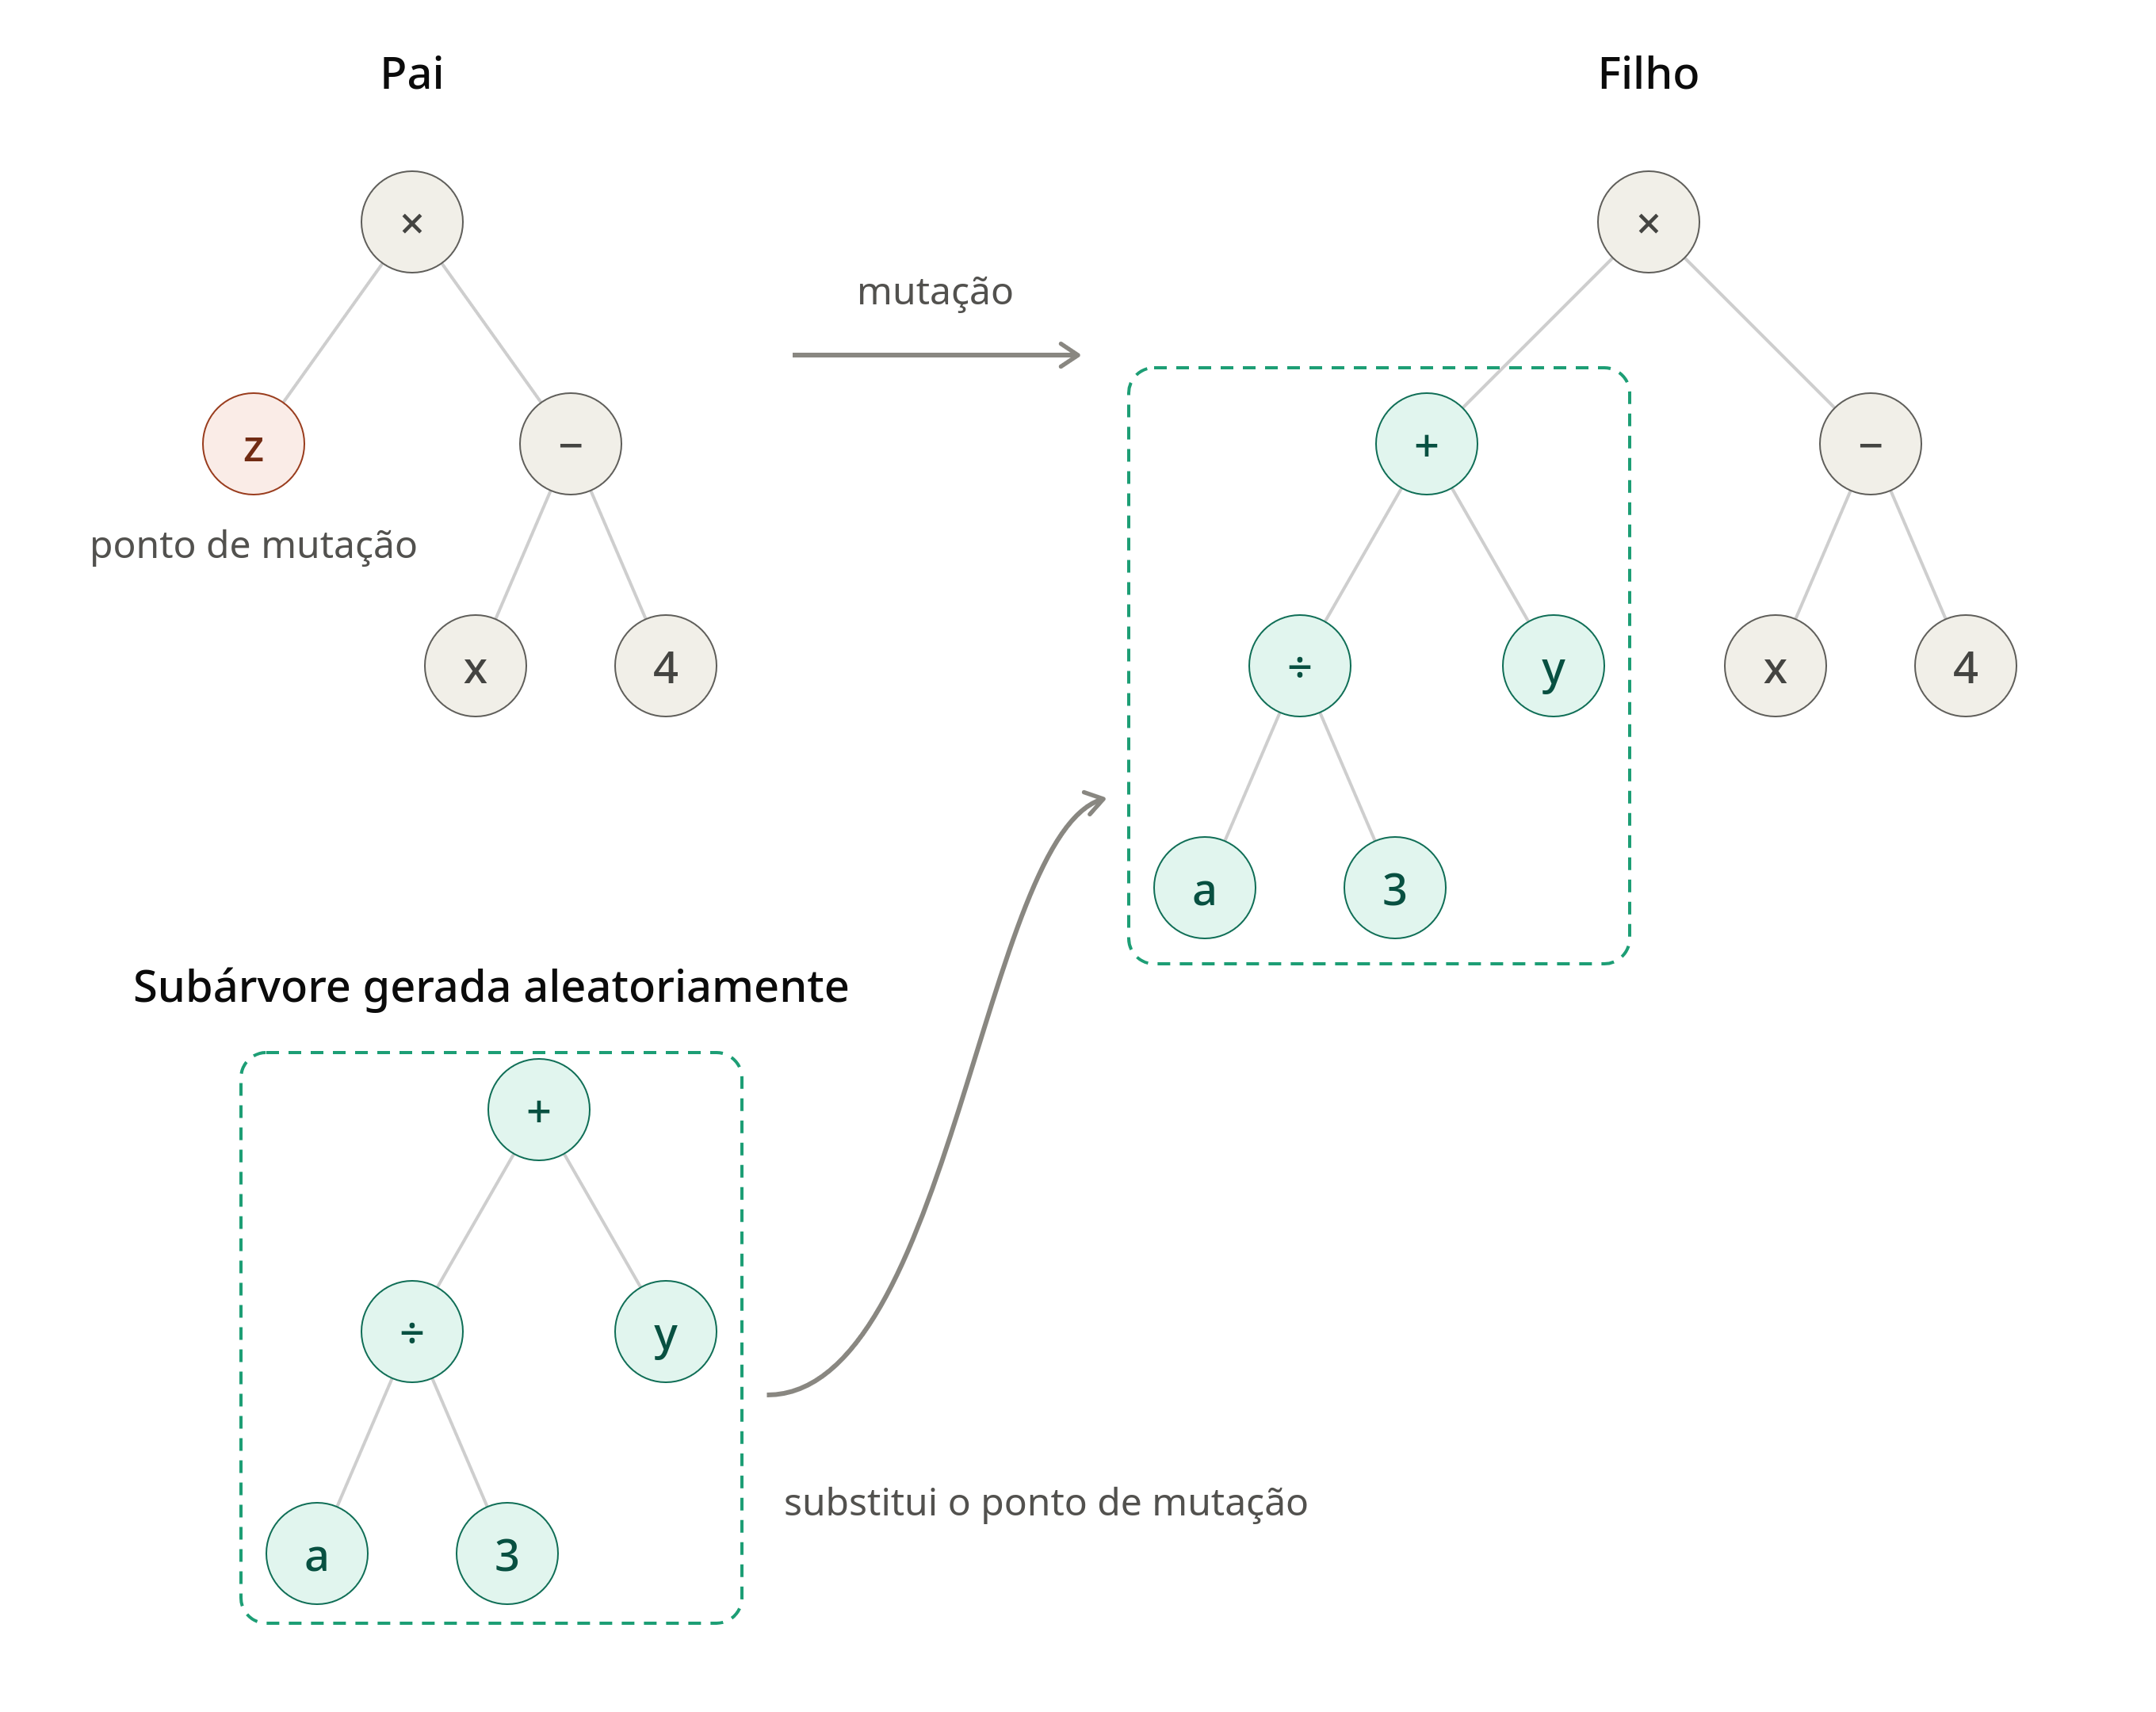
\includegraphics[width=\linewidth]{imgs/mutacao.png}
          \caption{Operador de mutação. Adaptado de \cite{fieldguide}}
          \label{fig:mut}
      \end{figure}
    \end{column}
  \end{columns}
\end{frame}

\subsection{\textit{General Program Synthesis Benchmark Suite}}
\begin{frame}{\textit{General Program Synthesis Benchmark Suite}}
  \begin{itemize}
    \item O \textit{General Program Synthesis Benchmark Suite}, ou PSB1,
      é um \textit{benchmark} que visa nivelar a avaliação de algoritmos de GP \cite{psb1}.
    \item Hoje muito usado na área \cite{psb2}.
    \item Problemas retirados de livros didáticos de introdução a computação.
    \item Especificação: exemplos.
  \end{itemize}
\end{frame}
\begin{frame}{\textit{General Program Synthesis Benchmark Suite}}
  \begin{examples}
    \textbf{Checksum:} dada uma string, converta cada caractere na string em
    seu valor ASCII inteiro, some-os, tome a soma módulo $64$,
    adicione o valor do inteiro correspondente ao caractere de espaço,
    e então converta esse inteiro de volta ao seu caractere correspondente
    (o caractere de \textit{checksum}).
    O programa deve imprimir \texttt{Check sum is X},
    onde $X$ é substituído pelo valor correto do caractere de \textit{checksum}.
  \end{examples}
\end{frame}

\section{Introdução}
\begin{frame}{Motivação}
  \begin{itemize}
    \item GP é uma técnica que consegue produzir resultados comparáveis com
      os de humanos \cite{fieldguide}.
    \item Há uma premiação para
      resultados gerados por GP e computação evolutiva \cite{humies}.
    \item É desejável avaliar o estado da literatura de GP e comparar técnicas.
  \end{itemize}
\end{frame}

\begin{frame}{Objetivos do \textit{survey}}
  \begin{itemize}
    \item No \textit{survey} \cite{survey}, os autores buscam descobrir o seguinte:
  \end{itemize}
  \begin{enumerate}
    \item Quais são as técnicas de GP mais relevantes na literatura?
    \item Como essas técnicas se comparam em termos de taxa de sucesso?
  \end{enumerate}
\end{frame}

\begin{frame}{Métodos}
  \begin{itemize}
    \item Filtrar artigos que citam o PSB1 diretamente.
    \item Comparar taxas de acerto de artigos cujos dados estão disponíveis.
  \end{itemize}
\end{frame}


\subsection{Principais algoritmos}
\begin{frame}{\textit{Stack-based} GP}
  \begin{itemize}
    \item Compõe a maior quantidade de artigos no \textit{survey} (37 artigos).
    \item Expoente é o Push \cite{pushgp} e variantes.
    \item Linguagem projetada especificamente para GP.
    \item Programas são listas de instruções e literais.
    \item Um literal é depositado na pilha do seu tipo e uma instrução consome
      elementos das pilhas, empilhando seus resultados.
  \end{itemize}
  \begin{examples}
    \texttt{(3 4 INTEGER.+) (1 2 INTEGER.+) INTEGER./}
  \end{examples}
\end{frame}
\begin{frame}{\textit{Stack-based} GP}
  \begin{figure}
      \centering
      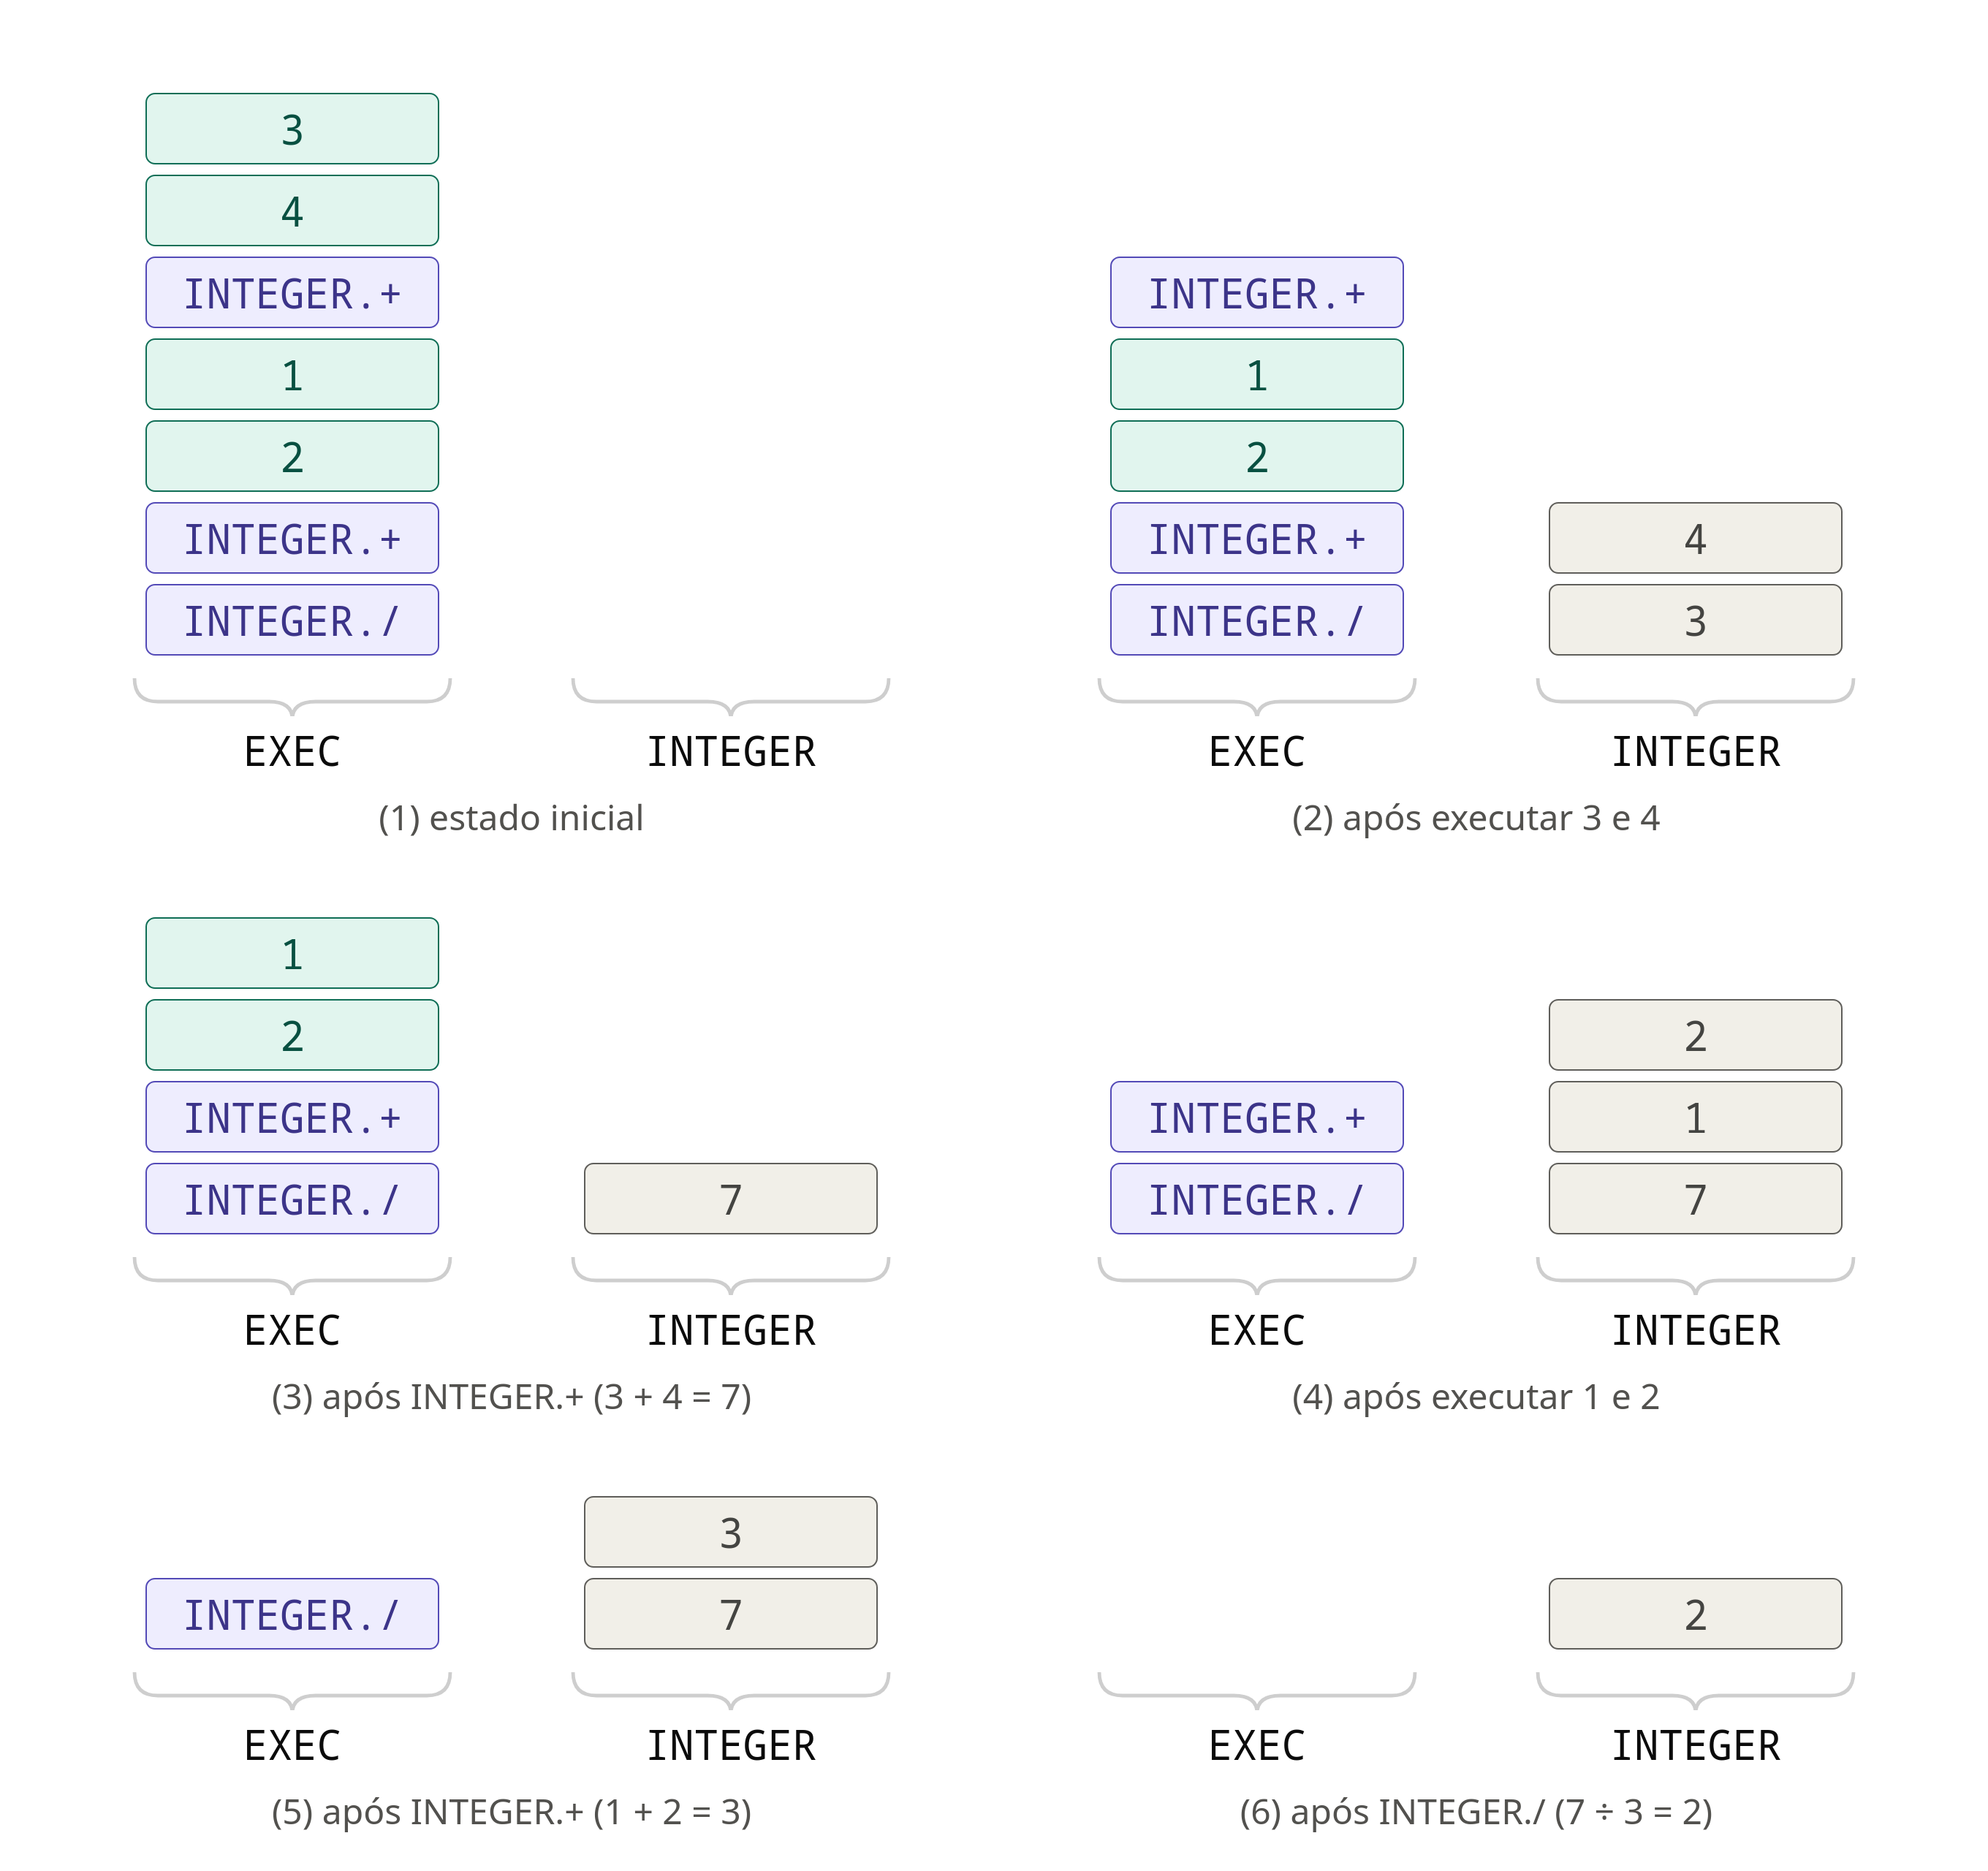
\includegraphics[height=0.8\textheight]{imgs/push_exec.png}
      \caption{Execução de um programa Push. Adaptado de \cite{survey}}
      \label{fig:push}
  \end{figure}
\end{frame}

\begin{frame}{\textit{Grammar-guided} GP}
  \begin{itemize}
    \item Segundo maior grupo de algoritmos (12 artigos).
    \item \textit{Grammatical Evolution} (GE) \cite{gramevo} e seus descendentes
    \item Dois componentes: uma gramática livre de contexto e uma lista de números.
    \item A partir de um \textit{scaffold}, escolhemos o ``buraco''
      mais a esquerda disponível.
    \item Dada uma quantidade $p$ de possíveis instruções e o primeiro número $n$
      da lista de números, escolhemos a solução de número $n \mod p$.
  \end{itemize}
\end{frame}

% gramatica_beamer.tex
% Slide da gramática (problema Smallest, versão simplificada).
% Inclua no main.tex com % gramatica_beamer.tex
% Slide da gramática (problema Smallest, versão simplificada).
% Inclua no main.tex com % gramatica_beamer.tex
% Slide da gramática (problema Smallest, versão simplificada).
% Inclua no main.tex com \input{gramatica_beamer} ou \include{gramatica_beamer}.
% Não precisa de pacotes extras: só do \usepackage[T1]{fontenc} (já presente
% no main), para que < e > saiam corretos em fonte monoespaçada.

% Token especial (NEWLINE, INDENT) em negrito sem serifa
\providecommand{\tok}[1]{\mbox{\textsf{\textbf{#1}}}}
% Barra que separa as alternativas da BNF
\providecommand{\ou}{$\mid$\ }

\begin{frame}{\textit{Grammar-guided} GP}
  \begin{figure}
  \centering
  \begin{examples}
  \small
  \ttfamily
  \setlength{\tabcolsep}{4pt}
  \renewcommand{\arraystretch}{1.35}
  \begin{tabular}{@{}l l l@{}}
    &n = &[13, 17, 7, 24, 21, 20, 18, 28, 4, 29] \\
    <program>  & ::= & def sum(int1, int2): \tok{NEWLINE} \tok{INDENT} \\
               &     & int3 = int() \tok{NEWLINE} \\
               &     & <stmt> return <int> \\
    <stmt>     & ::= & <stmt><stmt> \\
               & \ou & <int\_var> = <int> \tok{NEWLINE} \\
    <int\_var> & ::= & int1 \ou int2 \ou int3 \\
    <int\_op>  & ::= & + \ou - \ou * \ou / \ou \% \\
    <int>      & ::= & <int\_var> \\
               & \ou & <int> <int\_op> <int> \\
  \end{tabular}
  \end{examples}
  \caption{Exemplo de uma derivação de programa GE. Adaptado de \cite{survey}.}
  \end{figure}
\end{frame}
 ou % gramatica_beamer.tex
% Slide da gramática (problema Smallest, versão simplificada).
% Inclua no main.tex com \input{gramatica_beamer} ou \include{gramatica_beamer}.
% Não precisa de pacotes extras: só do \usepackage[T1]{fontenc} (já presente
% no main), para que < e > saiam corretos em fonte monoespaçada.

% Token especial (NEWLINE, INDENT) em negrito sem serifa
\providecommand{\tok}[1]{\mbox{\textsf{\textbf{#1}}}}
% Barra que separa as alternativas da BNF
\providecommand{\ou}{$\mid$\ }

\begin{frame}{\textit{Grammar-guided} GP}
  \begin{figure}
  \centering
  \begin{examples}
  \small
  \ttfamily
  \setlength{\tabcolsep}{4pt}
  \renewcommand{\arraystretch}{1.35}
  \begin{tabular}{@{}l l l@{}}
    &n = &[13, 17, 7, 24, 21, 20, 18, 28, 4, 29] \\
    <program>  & ::= & def sum(int1, int2): \tok{NEWLINE} \tok{INDENT} \\
               &     & int3 = int() \tok{NEWLINE} \\
               &     & <stmt> return <int> \\
    <stmt>     & ::= & <stmt><stmt> \\
               & \ou & <int\_var> = <int> \tok{NEWLINE} \\
    <int\_var> & ::= & int1 \ou int2 \ou int3 \\
    <int\_op>  & ::= & + \ou - \ou * \ou / \ou \% \\
    <int>      & ::= & <int\_var> \\
               & \ou & <int> <int\_op> <int> \\
  \end{tabular}
  \end{examples}
  \caption{Exemplo de uma derivação de programa GE. Adaptado de \cite{survey}.}
  \end{figure}
\end{frame}
.
% Não precisa de pacotes extras: só do \usepackage[T1]{fontenc} (já presente
% no main), para que < e > saiam corretos em fonte monoespaçada.

% Token especial (NEWLINE, INDENT) em negrito sem serifa
\providecommand{\tok}[1]{\mbox{\textsf{\textbf{#1}}}}
% Barra que separa as alternativas da BNF
\providecommand{\ou}{$\mid$\ }

\begin{frame}{\textit{Grammar-guided} GP}
  \begin{figure}
  \centering
  \begin{examples}
  \small
  \ttfamily
  \setlength{\tabcolsep}{4pt}
  \renewcommand{\arraystretch}{1.35}
  \begin{tabular}{@{}l l l@{}}
    &n = &[13, 17, 7, 24, 21, 20, 18, 28, 4, 29] \\
    <program>  & ::= & def sum(int1, int2): \tok{NEWLINE} \tok{INDENT} \\
               &     & int3 = int() \tok{NEWLINE} \\
               &     & <stmt> return <int> \\
    <stmt>     & ::= & <stmt><stmt> \\
               & \ou & <int\_var> = <int> \tok{NEWLINE} \\
    <int\_var> & ::= & int1 \ou int2 \ou int3 \\
    <int\_op>  & ::= & + \ou - \ou * \ou / \ou \% \\
    <int>      & ::= & <int\_var> \\
               & \ou & <int> <int\_op> <int> \\
  \end{tabular}
  \end{examples}
  \caption{Exemplo de uma derivação de programa GE. Adaptado de \cite{survey}.}
  \end{figure}
\end{frame}
 ou % gramatica_beamer.tex
% Slide da gramática (problema Smallest, versão simplificada).
% Inclua no main.tex com % gramatica_beamer.tex
% Slide da gramática (problema Smallest, versão simplificada).
% Inclua no main.tex com \input{gramatica_beamer} ou \include{gramatica_beamer}.
% Não precisa de pacotes extras: só do \usepackage[T1]{fontenc} (já presente
% no main), para que < e > saiam corretos em fonte monoespaçada.

% Token especial (NEWLINE, INDENT) em negrito sem serifa
\providecommand{\tok}[1]{\mbox{\textsf{\textbf{#1}}}}
% Barra que separa as alternativas da BNF
\providecommand{\ou}{$\mid$\ }

\begin{frame}{\textit{Grammar-guided} GP}
  \begin{figure}
  \centering
  \begin{examples}
  \small
  \ttfamily
  \setlength{\tabcolsep}{4pt}
  \renewcommand{\arraystretch}{1.35}
  \begin{tabular}{@{}l l l@{}}
    &n = &[13, 17, 7, 24, 21, 20, 18, 28, 4, 29] \\
    <program>  & ::= & def sum(int1, int2): \tok{NEWLINE} \tok{INDENT} \\
               &     & int3 = int() \tok{NEWLINE} \\
               &     & <stmt> return <int> \\
    <stmt>     & ::= & <stmt><stmt> \\
               & \ou & <int\_var> = <int> \tok{NEWLINE} \\
    <int\_var> & ::= & int1 \ou int2 \ou int3 \\
    <int\_op>  & ::= & + \ou - \ou * \ou / \ou \% \\
    <int>      & ::= & <int\_var> \\
               & \ou & <int> <int\_op> <int> \\
  \end{tabular}
  \end{examples}
  \caption{Exemplo de uma derivação de programa GE. Adaptado de \cite{survey}.}
  \end{figure}
\end{frame}
 ou % gramatica_beamer.tex
% Slide da gramática (problema Smallest, versão simplificada).
% Inclua no main.tex com \input{gramatica_beamer} ou \include{gramatica_beamer}.
% Não precisa de pacotes extras: só do \usepackage[T1]{fontenc} (já presente
% no main), para que < e > saiam corretos em fonte monoespaçada.

% Token especial (NEWLINE, INDENT) em negrito sem serifa
\providecommand{\tok}[1]{\mbox{\textsf{\textbf{#1}}}}
% Barra que separa as alternativas da BNF
\providecommand{\ou}{$\mid$\ }

\begin{frame}{\textit{Grammar-guided} GP}
  \begin{figure}
  \centering
  \begin{examples}
  \small
  \ttfamily
  \setlength{\tabcolsep}{4pt}
  \renewcommand{\arraystretch}{1.35}
  \begin{tabular}{@{}l l l@{}}
    &n = &[13, 17, 7, 24, 21, 20, 18, 28, 4, 29] \\
    <program>  & ::= & def sum(int1, int2): \tok{NEWLINE} \tok{INDENT} \\
               &     & int3 = int() \tok{NEWLINE} \\
               &     & <stmt> return <int> \\
    <stmt>     & ::= & <stmt><stmt> \\
               & \ou & <int\_var> = <int> \tok{NEWLINE} \\
    <int\_var> & ::= & int1 \ou int2 \ou int3 \\
    <int\_op>  & ::= & + \ou - \ou * \ou / \ou \% \\
    <int>      & ::= & <int\_var> \\
               & \ou & <int> <int\_op> <int> \\
  \end{tabular}
  \end{examples}
  \caption{Exemplo de uma derivação de programa GE. Adaptado de \cite{survey}.}
  \end{figure}
\end{frame}
.
% Não precisa de pacotes extras: só do \usepackage[T1]{fontenc} (já presente
% no main), para que < e > saiam corretos em fonte monoespaçada.

% Token especial (NEWLINE, INDENT) em negrito sem serifa
\providecommand{\tok}[1]{\mbox{\textsf{\textbf{#1}}}}
% Barra que separa as alternativas da BNF
\providecommand{\ou}{$\mid$\ }

\begin{frame}{\textit{Grammar-guided} GP}
  \begin{figure}
  \centering
  \begin{examples}
  \small
  \ttfamily
  \setlength{\tabcolsep}{4pt}
  \renewcommand{\arraystretch}{1.35}
  \begin{tabular}{@{}l l l@{}}
    &n = &[13, 17, 7, 24, 21, 20, 18, 28, 4, 29] \\
    <program>  & ::= & def sum(int1, int2): \tok{NEWLINE} \tok{INDENT} \\
               &     & int3 = int() \tok{NEWLINE} \\
               &     & <stmt> return <int> \\
    <stmt>     & ::= & <stmt><stmt> \\
               & \ou & <int\_var> = <int> \tok{NEWLINE} \\
    <int\_var> & ::= & int1 \ou int2 \ou int3 \\
    <int\_op>  & ::= & + \ou - \ou * \ou / \ou \% \\
    <int>      & ::= & <int\_var> \\
               & \ou & <int> <int\_op> <int> \\
  \end{tabular}
  \end{examples}
  \caption{Exemplo de uma derivação de programa GE. Adaptado de \cite{survey}.}
  \end{figure}
\end{frame}
.
% Não precisa de pacotes extras: só do \usepackage[T1]{fontenc} (já presente
% no main), para que < e > saiam corretos em fonte monoespaçada.

% Token especial (NEWLINE, INDENT) em negrito sem serifa
\providecommand{\tok}[1]{\mbox{\textsf{\textbf{#1}}}}
% Barra que separa as alternativas da BNF
\providecommand{\ou}{$\mid$\ }

\begin{frame}{\textit{Grammar-guided} GP}
  \begin{figure}
  \centering
  \begin{examples}
  \small
  \ttfamily
  \setlength{\tabcolsep}{4pt}
  \renewcommand{\arraystretch}{1.35}
  \begin{tabular}{@{}l l l@{}}
    &n = &[13, 17, 7, 24, 21, 20, 18, 28, 4, 29] \\
    <program>  & ::= & def sum(int1, int2): \tok{NEWLINE} \tok{INDENT} \\
               &     & int3 = int() \tok{NEWLINE} \\
               &     & <stmt> return <int> \\
    <stmt>     & ::= & <stmt><stmt> \\
               & \ou & <int\_var> = <int> \tok{NEWLINE} \\
    <int\_var> & ::= & int1 \ou int2 \ou int3 \\
    <int\_op>  & ::= & + \ou - \ou * \ou / \ou \% \\
    <int>      & ::= & <int\_var> \\
               & \ou & <int> <int\_op> <int> \\
  \end{tabular}
  \end{examples}
  \caption{Exemplo de uma derivação de programa GE. Adaptado de \cite{survey}.}
  \end{figure}
\end{frame}

\begin{frame}{\textit{Grammar-guided} GP}
  \begin{figure}
      \centering
      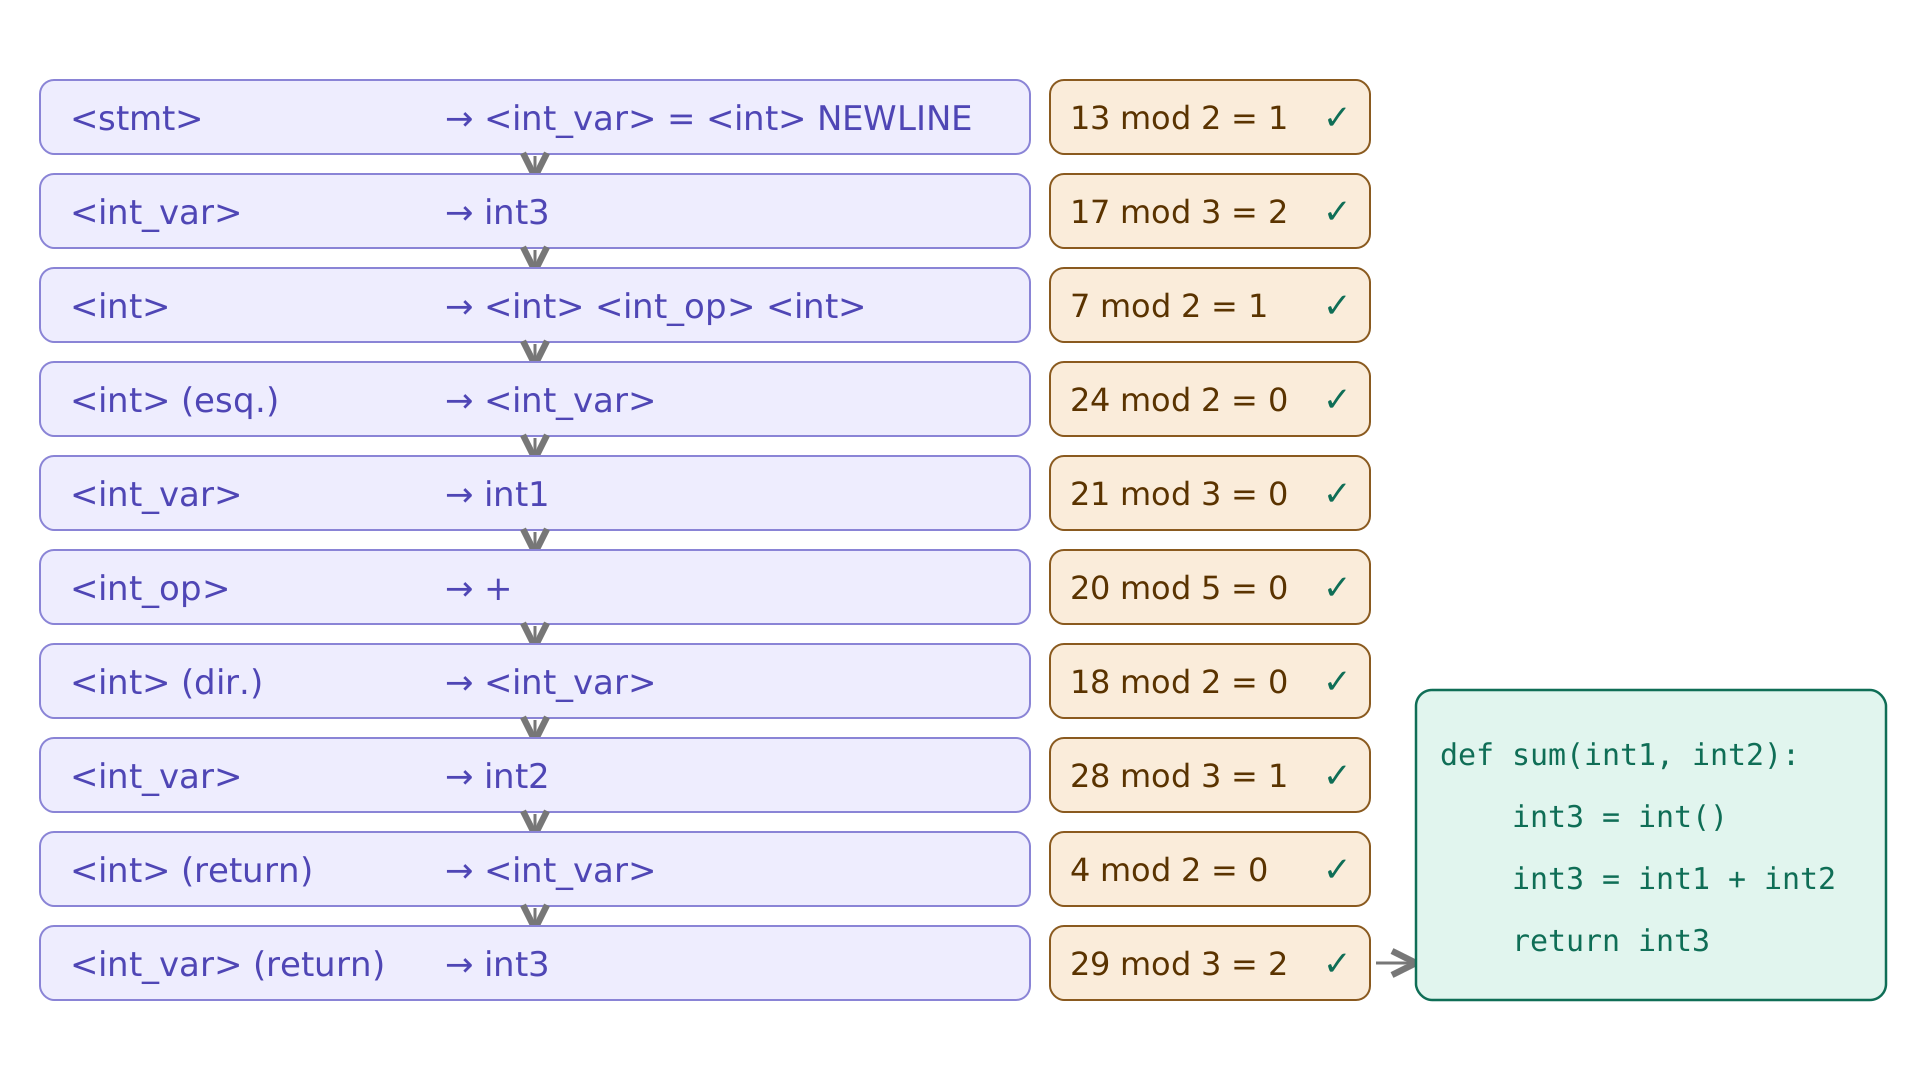
\includegraphics[width=0.9\linewidth]{imgs/g3p_derivation.png}
      \caption{Exemplo de uma derivação de programa GE. Adaptado de \cite{survey}.}
      \label{fig:g3pderiv}
  \end{figure}
\end{frame}

\begin{frame}{Outros algoritmos}
  \begin{itemize}
    \item Destaque: \textit{Linear GP} \cite{lineargp} (5 artigos).
    \item Semelhante a Assembly
    \item Consiste de uma série de registradores, os quais literais podem ser
      carregados ou guardados.
    \item Instruções manipulam o conteúdo dos registradores
  \end{itemize}
\end{frame}

\subsection{Desempenho no PSB1}
% tabela_beamer.tex -- fragmento (sem preâmbulo), incluído por main.tex via \input.
% Requer no preâmbulo de main.tex: xcolor=table, booktabs, multirow, pifont,
% \cmark, \xmark, \cabecalho e \legenda.

% ---------- Slide 1/3 ----------
\begin{frame}{Taxa de sucesso por problema (1/3)}
  \centering
  \small
  \renewcommand{\arraystretch}{1.15}
  \rowcolors{3}{}{gray!15}
  \begin{tabular}{lccc}
    \cabecalho
    Number IO                   & 96.0 (12.0) & 100 & \xmark \\
    Smallest                    & 78.0 (50.0) & 100 & \xmark \\
    Mirror Image                & 71.5 (75.0) & 100 & \cmark \\
    Median                      & 62.0 (39.5) & 100 & \xmark \\
    Negative to Zero            & 58.0 (60.0) & 98  & \cmark \\
    Replace Space with Newline  & 51.0 (56.0) & 100 & \cmark \\
    For Loop Index              & 40.0 (53.5) & 88  & \cmark \\
    String Lengths Backwards    & 35.0 (57.0) & 100 & \cmark \\
    Vector Average              & 32.5 (72.25) & 100 & \cmark \\
    Last Index of Zero          & 30.0 (40.0) & 96  & \cmark \\
    \bottomrule
  \end{tabular}
  \legenda
\end{frame}

% ---------- Slide 2/3 ----------
\begin{frame}{Taxa de sucesso por problema (2/3)}
  \centering
  \small
  \renewcommand{\arraystretch}{1.15}
  \rowcolors{3}{}{gray!15}
  \begin{tabular}{lccc}
    \cabecalho
    Grade                       & 23.2 (67.5) & 100 & \xmark \\
    Compare String Lengths      & 20.0 (38.75) & 95 & \cmark \\
    Syllables                   & 12.5 (19.5) & 76  & \cmark \\
    Digits                      & 10.0 (28.0) & 100 & \cmark \\
    Vectors Summed              & 7.5 (18.5)  & 93  & \cmark \\
    Sum of Squares              & 7.0 (12.25) & 41  & \cmark \\
    X-Word Lines                & 6.0 (56.75) & 98  & \cmark \\
    Small or Large              & 6.0 (7.5)   & 92  & \xmark \\
    Count Odds                  & 5.0 (10.0)  & 22  & \cmark \\
    Scrabble Score              & 4.0 (17.0)  & 90  & \cmark \\
    \bottomrule
  \end{tabular}
  \legenda
\end{frame}

% ---------- Slide 3/3 ----------
\begin{frame}{Taxa de sucesso por problema (3/3)}
  \centering
  \small
  \renewcommand{\arraystretch}{1.15}
  \rowcolors{3}{}{gray!15}
  \begin{tabular}{lccc}
    \cabecalho
    Super Anagrams              & 2.0 (25.0)  & 82  & \cmark \\
    Double Letters              & 1.0 (16.0)  & 87  & \cmark \\
    Checksum                    & 0.0 (1.0)   & 56  & \cmark \\
    Even Squares                & 0.0 (1.0)   & 15  & \cmark \\
    Pig Latin                   & 0.0 (0.0)   & 5   & \cmark \\
    String Differences          & 0.0 (0.0)   & 1   & \cmark \\
    Collatz Numbers             & 0.0 (0.0)   & 0   & \cmark \\
    Wallis Pi                   & 0.0 (0.0)   & 0   & \cmark \\
    Word Stats                  & 0.0 (0.0)   & 0   & \cmark \\
    \bottomrule
  \end{tabular}
  \legenda
\end{frame}

\begin{frame}{Desempenho no PSB1}
  \begin{itemize}
    \item Ao analisar os dados de desempenho, os autores notaram o seguinte \cite{survey}:
    \item Não há um algoritmo de GP que domine o outro; todos têm pontos
      fortes e são os melhores em algum problema.
    \item Apesar de alguns algoritmos acharem soluções perfeitas para alguns
      dos problemas do PSB1, há grande variação de resultados, especialmente
      em problemas mais ``difíceis''.
    \item No geral, problemas que requerem iteração/recursão, múltiplos subproblemas
      ou mudança de tipos apresentam desempenho ruim para todos os algoritmos.
  \end{itemize}
\end{frame}

\subsection{Conclusão}
\begin{frame}{Conclusão}
  \begin{itemize}
    \item Os autores convidam os pesquisadores da área a desenvolver técnicas
      que lidem melhor com problemas recursivos, bem como problemas compostos
      por subproblemas.
    \item Também ressaltam que, apesar dos resultados, programas gerados por
      GP devem ser mais parecidos com programas escritos por humanos para serem
      adotados de modo mais amplo.
  \end{itemize}
\end{frame}

\section{Críticas}
\begin{frame}{Críticas}
  \begin{itemize}
    \item Nenhuma crítica feita pelos autores à metodologia e qualidade
      dos dados disponíveis na literatura.
    \item Nenhuma crítica feita pelos autores à falta de outros tipos de dados
      relevantes (qualidade das soluções, comprimento das soluções, tempo total
      de execução dos experimentos, ambiente de execução, etc).
  \end{itemize}
\end{frame}

\begin{frame}[allowframebreaks]
    \frametitle{Referências}

    \bibliographystyle{apalike}
    \bibliography{references}
\end{frame}
\end{document}
